\documentclass[11pt,a4paper,oneside]{memoir}
\usepackage[latin1]{inputenc}
\usepackage[T1]{fontenc}
\usepackage[finnish]{babel}
\usepackage{amsmath}
\usepackage{amsfonts}
\usepackage{amssymb}
\usepackage{fontspec}
\usepackage{tocloft}
\usepackage{lipsum}
\usepackage{titlesec}
\usepackage{url}
\usepackage{mathtools}
\usepackage{float}

%\usepackage{hyperref}
%condition for adding or not space in TOC
\usepackage{etoolbox}
%for compact list
\usepackage{enumitem}
%for block comment
\usepackage{verbatim}
%for "easier" references
\usepackage{varioref}
%forcing single line spacing in bibliography
\DisemulatePackage{setspace}
\usepackage{setspace}
%including figure (image)
\usepackage{graphicx}
%change the numbering for figure
\usepackage{chngcntr}
%strike trough
\usepackage{ulem}
%euro symbol
\usepackage{eurosym}

%NORMAL TEXT
%all text, title, etc. in same tahoma font
\setmainfont{Tahoma}
%line space
\linespread{1.5}
%\doublespacing
%margin
\usepackage[top=2.5cm, bottom=3cm, left=4cm, right=2cm, nofoot]{geometry}
\setlength{\parindent}{0pt}%first line of paragraph not indented
\setlength{\parskip}{16.5pt}%one empty line to separate paragraph
%list with small line space separation
\tightlists

%IMAGE - FIGURE
%the figures are in "illustration" folder.
\graphicspath{{illustration/}}
%figure number without chapter (1.1, 1.2, 2.1) to (1, 2, 3)
\counterwithout{figure}{chapter}
%border around images
\setlength\fboxsep{0pt}
\setlength\fboxrule{0.5pt}
%caption font size
\captionnamefont{\small}
\captiontitlefont{\small}
%space after figure caption (and other float elements)
\setlength{\belowcaptionskip}{-7pt}

%CODE
\newfloat{program}{thp}{lop}
\floatname{program}{Esimerkkikoodi}

%TOC
%remove dots.
\renewcommand*{\cftdotsep}{\cftnodots}
%chapter title and page number not in bold.
\renewcommand{\cftchapterfont}{}
\renewcommand{\cftchapterpagefont}{}
%sub section in toc
\setcounter{tocdepth}{2}
%subsection numbered
\setcounter{secnumdepth}{2}
%\cfttoctitlefont{\normalfont\MakeUppercase}
\renewcommand{\tocheadstart}{\vspace*{-15pt}}
\renewcommand{\printtoctitle}[1]{\fontsize{13pt}{13pt}\bfseries #1}
\renewcommand{\aftertoctitle}{\vspace*{-22pt}\afterchaptertitle}
%spacing afer a chapter in toc
\preto\section{%
  \ifnum\value{section}=0\addtocontents{toc}{\vskip11pt}\fi
}
%spacing afer a section in toc
\renewcommand{\cftsectionaftersnumb}{\vspace*{-3pt}}
%spacing afer a subsection in toc
\renewcommand{\cftsubsectionaftersnumb}{\vspace*{-1pt}}

%TITLES
%chapter title
\titleformat{\chapter}
{\fontsize{13pt}{13pt}\bfseries\linespread{1}}
{\thechapter}{.5cm}{}
\titlespacing*{\chapter}{0pt}{.32cm}{9pt}
\titleformat{\section}
{\fontsize{12pt}{12pt}\linespread{1}}
{\thesection}{.5cm}{}
\titlespacing*{\section}{0pt}{14pt}{6pt}
\titleformat{\subsection}
{\fontsize{12pt}{12pt}\linespread{1}}
{\thesubsection}{.5cm}{}
\titlespacing*{\subsection}{0pt}{14pt}{6pt}

%QUOTE
\renewenvironment{quote}
    {\list{}{\rightmargin=0pt\leftmargin=1cm\topsep=-10pt}%
    \item\relax\fontsize{10pt}{10pt}\singlespacing}
    {\endlist}

%BIBLIOGRAPHY
%bibliography title to be "references"
\renewcommand\bibname{References}
\makeatletter % Reference list option change
\renewcommand\@biblabel[1]{#1\hspace{1cm}} % from [1] to 1 with 1cm gap
\makeatother %
%\makeatletter %
%\renewcommand\@bibitem{\linespread{0.5}} %
%\makeatother %
%\setlength{\bibitem}{16.5pt}
\setlength{\bibitemsep}{11pt}

\author{Panu Leppäniemi}
\title{Automaattinen keskustelun visualisointi}

%==============================================================================
\begin{document}
%page number always on the top right. And clear the "chapter/section" head.
\pagestyle{myheadings}
\markright{}
%clear chapter "title" foot page.
\makeevenfoot{plain}{}{}{}
\makeoddfoot{plain}{}{}{}

%title page comes here...

%abstract comes here...

%==============================================================================
\makeevenhead{plain}{}{}{}
\makeoddhead{plain}{}{}{}
\pagestyle{empty} %remove page number in toc (if longer than 2 pages)
\tableofcontents*
\pagestyle{empty} %remove page number in toc (if longer than 1 pages)
\clearpage
\pagestyle{plain}

%list of figure, tables comes here...

%abbreviation comes here...

%page number always on top right; also for chapter "title" page
\makeevenhead{plain}{}{}{\thepage}
\makeoddhead{plain}{}{}{\thepage}

\setcounter{page}{1} %page 1 should be Introduction

%==============================================================================
\chapter{Johdanto}
Tavoitteena on selvittää, voiko keskustelun automaattisesta visualisoinnista ja yhteenvedosta olla hyötyä keskustelun kokonaisuuden hahmottamisen suhteen. Samalla todennetaan insinöörityössä hyödynnettävän Juju-ohjelmiston käyttökelpoisuus.

\chapter{Keskustelijoiden vuorovaikutus keskusteluun ja toisiinsa}
Keskustelun osalliset ja heidän väliset suhteet vaikuttavat keskustelun kulkuun ja lopputulokseen. Mielenkiinnon kohteet keskustelussa vaihtelevat osallisten kontribuutiolla. \cite[s. 1]{finding-topics-in-dynamical-text}
...

Auttaako visualisointi dialektiikan eli keskinäisviestinnän todentamisessa? Puhuvatko ihmiset siis samoista asioista, vai ilmaisevatko he omia ajatuksiaan sivuuttaen keskustelukumppanin sanoman?

Kenen aloittamista aiheista puhutaan? Kenellä on ollut valtaa ohjata keskustelun kulkua? Kuka tuo keskusteluun uutta sisältöä ja kuka toistelee aikaisemman keskustelun asettamia teemoja?

Onko keskustelun sisältö helpompi hahmottaa, kun siitä on etukäteen tehty automaattinen yhteenveto?

?????

Jos nähdään, mitä aiheita esimerkiksi palaverin aikana on käsitelty ja samalla kerätään huomioita, mitä asioita palaverin ansiosta on päätetty, voidaan mahdollisesti useamman palaverin jälkeen alkaa muodostaa mielikuvaa siitä, käsitelläänkö samaa aihetta useissa palavereissa saamatta aikaan mitään konkreettista. Näin voidaan nostaa esille mahdollisesti hankalat päätökset ja korottaa niiden painoarvoa seuraavassa käsittelyssä.

\chapter{Käyttötapaukset}

\section{Automaattinen litterointi - tulevaisuus}
Palavereissa, asiakastapaamisissa ja vastaavissa tilaisuuksissa vähintään yhden osallistujan kannattaa ottaa sihteerin rooli. Tämä tarkoittaa sitä, että hänen mahdollisuutensa osallistua keskusteluun vähenee merkittäväksi. Varsinkin pienemmässä projektiryhmässä yhden henkilön irroittaminen kyseiseen tehtävään ei aina ole mahdollista. Tunnetusti ihminen ei ole tehokas suorittamaan useita tehtäviä samanaikaisesti. Tämä saattaa johtaa siihen, ettei palaverin aikana kirjoitetun muistion laatu vastaa aina haluttua.

Yksi ratkaisuvaihtoehto on keskustelun äänittäminen muistiin, jolloin mikään käsitelty asia ei jäisi kirjaamatta. Näin vältettäisiin myös mahdolliset kiistatilanteet palaverin aikana tehdyissä suullisissa sopimuksissa. Ratkaisu on kuitenkin kömpelö, eikä soveltuisi varsinkaan pitkäkestoisiin keskusteluihin, koska nauhoituksen läpikäyminen jälkikäteen esimerkiksi yhteenvedon kirjoittamista varten veisi aikaa. Toiseksi voisi olla työlästä hahmottaa kuka vuorollaan on ollut äänessä, johtaen mahdollisiin väärinkäsityksiin.

Parempi ratkaisu tähän tilanteeseen voisi olla automaattinen litterointi. Puhe siis muutettaisiin automaattisesti tekstimuotoon. Automaatiolla vältettäisiin manuaalisen litteroinnin tulkinnanvaraisuudet.

Jatkuvan puheen muuttamiseksi tekstiksi on olemassa jo valmiita sovelluksia, esimerkiksi Nuance Communicationsin Dragon Dictation. Valitettavasti ongelmaksi muodostuu vielä toistaiseksi teknologian kehittymättömyys, joka johtaa  virhealttiuteen. Suurin osa varsinkin suomenkielisestä sovellustarjonnasta keskittyy yksinkertaiseen puheentunnistukseen, jota voidaan hyödyntää esimerkiksi puheohjauksessa. Tällainen sovellus on tehty tunnistamaan ennaltamääriteltyjä, usein yksiosaisia komentoja. Dragon Dictation -tuoteperheen englanninkielistä palvelinpuolen sovellusta olisi voitu hyödyntää insinöörityössä, mutta tiedon eristämisen koneisto, Juju, prosessoi ainoastaan suomenkieltä. Näin ollen automaattinen litterointi jää toistaiseksi teoriatasolle.

Kuvitellaan kuitenkin automaattisen litteroinnin olevan mahdollista. Jotta tallenteen analysointi olisi mielekästä keskustelun näkökulmasta, puheenvuoroihin pitäisi liittää identiteettitieto. Toistaiseksi tarvittavaa teknologiaa, joka puheen lisäksi tunnistaisi puhujan identiteetin luotettavasti, ei ole olemassa [SELVITÄ], joten tämä pitäisi korvata yksinkertaisemmalla ratkaisulla. Teknisesti helposti toteutettava vaihtoehto olisi jakaa keskustelun osallisille henkilökohtaiset mikrofonit. Mikrofoneihin liitettäisiin puhujan henkilöllisyys joko etu- tai jälkikäteen. Tämä helpottaisi huomattavasti keskustelun etenemisen hahmottamista.

Edellämainitun ratkaisun avulla pystyisimme keräämään keskustelusta taulukossa [TAULUKKO] esitetyn formaatin mukaista dataa. Järjestelmä olettaa, että saatavissa oleva aineisto on kyseisessä muodossa (CSV).

\begin{tabular}{| l | l | l |}
\hline
Aika & Henkilö & Puheenvuoro \\ \hline
2012-08-11 13:37 & Matti & Olipas kerran... \\ \hline
2012-08-11 16:20 & Teppo & Siinäpä tarinaa kerrakseen. Muistan kerran, kun... \\ \hline
2012-08-11 16:24 & Matti & Sepä kiva muistelma. \\ \hline
\end{tabular}

\chapter{Tekninen toteutus ja tietorakenteet}
Järjestelmän tekninen toteutus on joustavuuden nimissä jaettu selkeästi kahteen osaan: prosessointityökaluun ja käyttöliittymään (web-palvelu). Tämä mahdollistaa prosessointityökalun hyödyntämisen erillisissä palveluissa ilman, että se on sidottu mihinkään valmiiseen käyttöliittymään. Samalla web-palvelun voi julkaista tietokantaan tallennetulla esiprosessoidulla datalla. Rakenne on esitetty kuvassa [KUVA].

\section{Järjestelmien välinen viestintä}
Järjestelmän prosessointityökalu ja käyttöliittymä on toteutettu eri teknologioilla: Scala ja PHP. Tämä johtaa siihen, ettei järjestelmien välinen viestintä ole täysin yksiselitteistä. Tämä ei kuitenkaan ole ongelma, vaan ratkaisuja tähän ongelmaan on olemassa \vref{topic:amqp}.

Viestit välitetään järjestelmästä toiseen eri muodoissa. Ne käsitellään Base64-koodauksella riippumatta viestin kulkusuunnasta. Enkoodauksen tarkoituksena on välttää mahdolliset merkistöongelmat ja tästä mahdollisesti aiheutuva tiedon korruptoituminen. Lähettävä osapuoli enkoodaa viestin, ja vastaanottaja dekoodaa sen.

Käyttöliittymä lähettää palveluun ladatun CSV-tiedoston sisällön prosessointityökalulle. Tiedoston sisältöä ei vielä tässä vaiheessa prosessoida, lukuunottamatta enkoodausta.

Prosessointityökalu rakentaa viestijonon kautta saadusta CSV-materiaalista JSON-formaatin mukaista dataa. Tämä välitetään takaisin käyttöliittymäohjelmistolle tallennettavaksi tietokantaan. 

\subsection{Advanced Message Queue Protocol\label{topic:amqp}}
Viestijonoprotokollaa, AMQP, käytetään tiedon välittämiseen järjestelmästä toiseen. AMQP:n toteuttava middleware broker!! toimii viestinvälittäjänä.

Termistöstä??

Protokolla mahdollistaa myös sovelluksen jakamisen tarvittaessa useammalle palvelimelle. Edellämainitusta jaosta seuraa useitakin hyötyjä. Palvelinympäristöt on hyvä konfiguroida mahdollisimman yksinkertaisiksi ja asentaa vain ne sovellukset, joita projekti tarvitsee. Näin esimerkiksi tietoturvaa on helpompi ylläpitää, koska päivitettävien riippuvuuksien määrä on minimoitu. Samalla voidaan optimoida palvelinta suorituskyvyn kannalta juuri sille asetetun tehtävän mukaisesti.

Työssä on käytetty AMQP:n standardin toteuttavaa RabbitMQ-palvelinohjelmistoa. RabbitMQ on toteutettu funktionaalisella Erlang-ohjelmointikielellä. 

Erilaisia protokollan mukaisia viestimenetelmiä on muutama, jotka ovat (Exchange types):

- direct messaging
- asd asd
- asd asd 

Työhön on valittu käytettäväksi yksinkertaisin direct-menetelmä, koska se on käyttötapauksen kannalta riittävä.

\section{Prosessointi}
Prosessointityökalu pyörii ajastetusti tausta-ajona. Se on toteutettu hyödyntäen seuraavia teknologioita:

- Scala
- Java
- Akka.

Prosessointi höydyntää E-Reading -hankkeen yhteydessä toteutettua Juju-koneistoa.

\subsection{Juju}
Juju on Javalla toteutettu ohjelmisto, jota voidaan käyttää entiteettien tunnistamiseen ja avainsanojen poimintaan. Lähitulevaisuudessa Juju on tarkoitus julkaista avoimena lähdekoodina. Jujun kehitys on ollut pitkään kokeellista, mutta insinöörityön aikana koneistoa on viimeistelty. Työn aikana oli tarkoitus todentaa koneiston käyttökelpoisuus ulkopuolisen näkökulmasta. Samalla oli mahdollisuus vaikuttaa ohjelmiston rajapinnan, dokumentaation ja sen kehittämiseen liittyvien käytäntöjen kehitykseen.

Juju-integraation helpottamiseksi Juju konvertoitiin Maven-projektiksi. Aikaisemmin ulkoiset kirjastot, joihin Jujulla oli riippuvuus, säilytettiin versiohallinnassa erillisessä projektissa. Nykyään riippuvuudet on määritelty pom.xml-tiedostossa.

\begin{verbatim}
<dependencies>
    <dependency>
        <groupId>com.google.guava</groupId>
        <artifactId>guava</artifactId>
        <version>13.0.1</version>
    </dependency>
    ...
</dependencies>
\end{verbatim}
Esimerkki Jujun riippuvuuksien määrittelystä pom.xml-tiedostolla.

Edellämainittu konvertointi mahdollistaa Jujun integroinnin helposti muihin Maven- tai Mavenin pom-määritystä tukeviin projekteihin, kuten SBT-projektiin.

\subsection{Scala}
Scala on ohjelmointikieli, joka yhdistää kaksi tekijää yhteen, jotka yleensä nimenomaan erottavat kieliä toisistaan; olio-ohjelmoinnin ja funktionaalisen ohjelmoinnin. 
\cite[asd]{scala-by-example}
[Scala By Example, Martin Odersky, 2011]

Koska Scala toimii JVM:n päällä, sillä on mahdollista käyttää muilla ohjelmointikielillä toteutettuja ohjelmia, jotka käännetään JVM-yhteensopivaksi tavukoodiksi. Tämän ansiosta Javalla toteutetun Juju-kirjaston käyttöönotto projektissa oli helppoa.

\subsection{SBT}
SBT, Simple Build Tool, on pääasiassa Scala-projekteihin tarkoitettu nönnönnöö.

\begin{program}
  \begin{verbatim}
  resolvers += "Local Maven Repository" at "file://.m2/repository"
  libraryDependencies += "fi.metropolia.ereading" % "Juju" % "0.0.1-SNAPSHOT"
  \end{verbatim}
  \caption{Esimerkki Jujun määrityksestä projektiin riippuvuudeksi sbt.build-tiedostossa.}
\end{program}

Riippuvuuden määrittelyn jälkeen Juju voidaan ladata, jonka jälkeen se on valmis käytettäväksi.

\section{Käyttöliittymä}

\subsection{Symfony2}

\subsection{MongoDB}
MongoDB on dokumenttiorientoitunut tietokanta. 

\subsection{D3.js}
D3 on JavaScript-kirjasto.

\chapter{Visualisointi}
Keskustelun visualisoinnin tarkoituksena on helpottaa sisällön ja suhteiden hahmottamista.

- Kokonainen keskustelu on luettavissa
- Yksittäisten puheenvuorojen avainsanat esiintymisjärjestyksessä

\section{Asiasanoitus}
Työn aikana pyrittiin selvittämään, voiko keskustelun painopisteitä hahmottaa paremmin asiasanoittamalla puheenvuorot. 

Tarkkojen numeeristen arvojen esittämistä avainsanojen painotuksessa ei koettu hyödylliseksi, vaan painotus visualisoitiin suhteellisesti tekemällä tärkeiden sanojen elementeistä kooltaan isompia.

\section{Puheenvuorojen samanlaisuudet}
Haluttiin selvittää, onko puheenvuorojen samanlaisuuksien ja eroavaisuuksien seuraaminen hyödyllistä, tai voidaanko näitä visualisoimalla hahmottaa jotakin uutta keskusteluun liittyen. Pystytäänkö esimerkiksi erottelemaan keskustelijat, jotka kykenevät tuomaan uusia ideoita puheenaiheiksi heistä, jotka vain toistelevat edellämainittuja aiheita lisäämättä mitään uutta. Eroavaisuuksista voidaan myös mahdollisesti nähdä, eteneekö keskustelu eri aihepiireihin.

Työssä tutkittiin kahta erilaista lähestymistapaa:
\begin{enumerate}
\item puheenvuoron eroavaisuus verrattuna edelliseen puheenvuoroon
\item yksittäisen puheenvuoron eroavaisuus keskustelukokonaisuuteen.
\end{enumerate}

Samanlaisuuden tai erilaisuuden analysoimisessa voidaan käyttää useita eri  määrittelytapoja. Määrittelytavan valinta riippuu analysoitavan materiaalin luonteesta, eikä sitä voi suoraan tieteellisesti perustella \cite[s. 298]{encyclopedia-of-distances}.

\subsection{Laskennallinen samanlaisuus (Jaccard)}
Jaccard-samanlaisuutta (rinnastetaan usein Tanimoto-samanlaisuuteen \cite[s. 299]{encyclopedia-of-distances}) voidaan käyttää dokumenttien samanlaisuuden vertailuun. Jaccard-samanlaisuus voidaan määrittää seuraavalla kaavalla:

\begin{math}
J(X, Y) = \frac{| X \bigcap Y |}{| X \bigcup Y |},
\end{math}

jossa X ja Y edustavat sanajoukkoja. Laskutoimituksessa jaetaan joukkojen X ja Y intersektion tuottaman joukon koko samojen joukkojen unionin koolla. Tuloksena on Jaccard-indeksi (Paul Jaccard, 1901), joka kuvastaa joukkojen samanlaisuutta. Funktion mahdolliset tulokset ovat välillä 0.0 - 1.0, jossa 0 tarkoittaa täysin erilaisia ja 1 täysin samanlaisia dokumentteja. Kyseisen kaavan toteuttaminen Scalalla on yksinkertaista:

\begin{program}
  \begin{verbatim}
def index(a: Set[String], b: Set[String]): Double =
  a.intersect(b).size / a.union(b).size.asInstanceOf[Double]
  \end{verbatim}
  \caption{Jaccard-indeksin laskennan toteutus.}
\end{program}

Huomaa, että Set-tietorakenne voi sisältää vain yksilöllisiä merkkijonoja, joten sanojen duplikaattiesiintymät karsitaan pois. Tämä on tärkeää, koska duplikaattiesiintymät vääristäisivät tulosta.

Sanajoukkojen eroavaisuus, Jakkard-etäisyys, voidaan laskea edellistä kaavaa mukaillen:

\begin{math}
J_\delta(X, Y) = 1 - \frac{| X \bigcap Y |}{| X \bigcup Y |} = \frac{| X \bigcup Y | - | X \bigcap Y |}{| X \bigcup Y |}.
\end{math}

Lähestymistapoja vertailtavan aineiston valinnan suhteen on pari. Samanlaisuutta vertailtaessa voidaan käyttää:

\begin{enumerate}
\item kokonaista puheenvuoroa, jota verrataan koko keskusteluun
\item puheenvuorosta poimittuja avainsanoja, joita verrataan koko keskustelusta poimittuihin avainsanoihin.
\end{enumerate}

Työn aikana päädyttiin käyttämään puheenvuoron asiasanoitusta samanlaisuuden vertailun joukkona, jotta saadaan verrattua puheenvuorojen olennaisimpia osia keskenään. Puheenvuoron jokaisen yksittäisen sanan käyttäminen vertailussa vääristäisi tuloksia kielessä käytettyjen konjuktioiden seurauksena. Asiasanoituksia käytettäessä herää kysymys, kannattaako myös avainsanojen painotukset ottaa huomioon vertailussa.

Yksinkertaisen Jaccard-indeksin heikkous on sisällön painoarvoistamisen puute. Jaccard-indeksissä vertaillaan sanojen esiintymiä toisiin ottamatta huomioon frekvenssiä; kuinka usein jokin sana on esiintynyt. Näin voidaan päätyä hyvinkin vääristyneisiin tuloksiin. Esimerkki: keskustelija, Matti, puhuu pääosin aiheesta X, ja mainitsee kerran aiheen Y. Toinen keskustelun osallinen, Teppo, puhuu taas päinvastoin aiheesta Y, mainiten X:n vain harvoin. Jos tästä keskustelusta laskettaisiin Jaccard-indeksi avainsanojen perusteella, saataisiin edellämainitusta keskustelusta koostetuilla määrittelyjoukoilla Jakkard-indeksin funktion tulokseksi 1. Toisinsanoen Jakkard-indeksi tulkitsee dokumentit täysin samanlaisiksi, joka ei keskustelua tarkasteltaessa pidä paikkaansa.

Painotettu Jaccard-indeksi voidaan määrittää vektoreille X ja Y seuraavanlaisesti \cite[s. 2]{finding-the-jaccard-median}:

\begin{math}
  J(X, Y) = \left\{ 
  \begin{array}{l l}
	\frac{\sum^n_{i=1} min(X_i, Y_i)}{\sum^n_{i=1} max(X_i, Y_i)} & \quad \text{$jos$ } \sum^n_{i=1} max(X_i, Y_i) > 0,\\
	1 & \quad \text{$jos$ } \sum^n_{i=1} max(X_i, Y_i) = 0.\\	
  \end{array} \right.
\end{math}

Painotetussa ratkaisussa ei siis vain vertailla samanlaisuutta esiintyneiden sanojen perusteella, vaan otetaan huomioon myös esiintymisfrekvenssi.

\subsection{Asiasanoituksen visualisointiin perustuva samanlaisuus}


\section{Chernoffin naamat}
Eräs todella tärkeä osa kommunikaatiota on ilmaisun tyyli. Tällä tarkoitan esimerkiksi sitä, millä äänensävyllä asian ilmaisee. Keskustelun tulkitsemisessa tällä on iso rooli. Jos keskustelu vaikka muuttuu dramaattisesti, puhetyylistä voidaan saada osviittaa mahdollisesta syystä. Ilmaisuille on tehty oma merkintäkielensä, [SELVITÄ].

Kielteisyyden tai myönteisyyden ilmentäminen on hankalaa.

Sähköisessä keskustelussa keskustelun sävyä on kuitenkin melkein mahdotonta tulkita. Yksi vaihtoehto keskustelun visualisoinnissa on käyttää.

Chernoffin naamoissa on 18 erilaista kasvonpiirteen mallia, joihin kuuluu esimerkiksi seuraavat:
\begin{itemize}
\item{pään muoto}
\item{nenän pituus}
\item{silmien koko ja vinous}
\item{silmien epäkeskisyys ja erillisyys}
\item{kulmakarvat ja katseen suunta}
\item{suun kaarevuus, leveys ja korkeus.}
\end{itemize}

\begin{figure}[h]
    \centering
    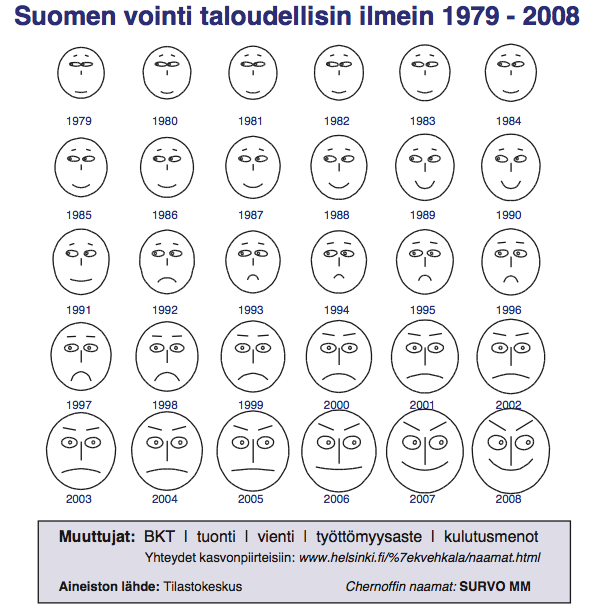
\includegraphics[width=10cm]{suomen-vointi-chernoff}
    \caption{Esimerkki Chernoffin naamoista: Suomen vointi taloudellisin ilmein \cite{wikibooks:latex}.}
    \label{fig:suomen-voint-chernoff}
\end{figure}

\section{Gamification}
Keskustelun pisteyttämisen ydintarkoitus on saada nopeasti karkea kuva osallistujien aktiivisuudesta ja puheenvuorojen laadukkuudesta. Pisteytys perustuu aina puheenvuoroon ja sen välisiin suhteisiin. Pisteitä saa esimerkiksi mainitsemalla uuden käsitteen keskustelun aikana.

Tämän lisäksi pisteyttämisen tuomalla "porkkanalla" voisi aktivoida osallistujia mukaan keskusteluun. Kyseinen ajatus liittyy Gamification-ajatusmalliin. Gamificationin perusidea on se, että pyritään tuomaan esimerkiksi videopeleistä tuttuja elementtejä arkipäivän rutiineihin, tarkoituksena motivoida työntekijää suoriutumaan tehtävistään.

Gamificationissa on myös mahdolliset haittapuolensa. Jos pisteytykselle annetaan liikaa painoarvoa, keskustelun osalliset saattavat keskittyä liikaa pisteiden keräämiseen. Tämä taas ohjaa pois laadukkaasta keskustelusta. Pisteytys on ulkoinen motivaation lähde, joka ei tuo mitään lisäarvoa itse keskusteluun. [The Dangers of Gamification, Krystle Jiang, 2011]

Mahdollisten riskien takia projektissa päädyttiin ratkaisuun, jossa pisteytystä ei ole yksityiskohtaisesti eroteltu tai korostettu. Sen sijaan pisteitä käytetään henkilön aktiivisuuden osoittamisen apuna.
...

\chapter{Tulosten todentaminen ja jatkokehitys}
Tällä hetkellä sovellus pyrkii olemaan kohtuullisen yleispätevä erikoistumatta mihinkään tiettyyn keskusteluvariaatioon. Jatkossa ohjelmistoa voisi jatkokehittää erikoistumaan erilaisiin sovellutuksiin. Eräs idea olisi hahmottaa yksittäisten henkilöiden välisten suhteiden lisäksi vuorovaikutusta isommassa mittakaavassa. Tämä voitaisiin saavuttaa erilaisten tunnisteiden lisäämisellä käsiteltävään materiaaliin. Yksi vaihtoehto olisi, että henkilölle määriteltäisiin ryhmä, johon hän kuuluu. Näin voitaisiin esimerkiksi politiikan viitekehyksessä havaita, miten puolueiden ajamat aihepiirit eroavat toisistaan.

Todennettiin, että Juju tuottaa tarpeeksi pätevää asiasanoitusta myös keskustelujen osalta.

%----------------------------------------------------------------------------------------
%   BIBLIOGRAPHY 
%----------------------------------------------------------------------------------------

\bibliographystyle{vancouver}
%line space
\singlespacing
\begin{flushleft}
\bibliography{biblio}
\end{flushleft}

\end{document}